\chapter{\rm\bfseries Probabilistic Program Repair}
\label{ch:chapter03}

As we have seen, the problem of program repair is highly underdetermined. To resolve this ambiguity, we will use a probabilistic model to induce a distribution over the language of valid programs. This distribution will guide the repair process by assigning a likelihood to each possible repair. Then, taking the maximum over all possible repairs, we can find the most likely repair consistent with the constraints and the observed program.

Specifically, we will define an ordering over strings by their likelihood under the probabilistic model. We then define a repair as the most likely string consistent with the observed program and the grammar. We factorize the probability of a string as the product of the probability of each token in the string, conditioned on its predecessors. This allows us to compute the joint probability in a left-to-right fashion.

This probabilistic model will generally admit programs that are locally probable, but globally inconsistent with the grammar. To enforce syntactic validity, we will use the probabilistic language model to ``steer'' a generative sampler through the automaton representing the repair language. This has two advantages: first, it allows us to sample from the repair language incrementally, and second, it ensures that subsequences with high probability are retrieved first, and all trajectories are syntactically valid.

We will consider two kinds of probabilistic models: a constrained Markov model and an unconstrained transformer-based neural network trained on program repair, then evaluate the performance of these models on a syntax repair benchmark consisting of pairwise program transformations. As we will show, the constrained Markov model is able to achieve state-of-the-art precision on blind prediction of the lexical sequence.

\begin{figure}[H]
  \resizebox{.24\textwidth}{!}{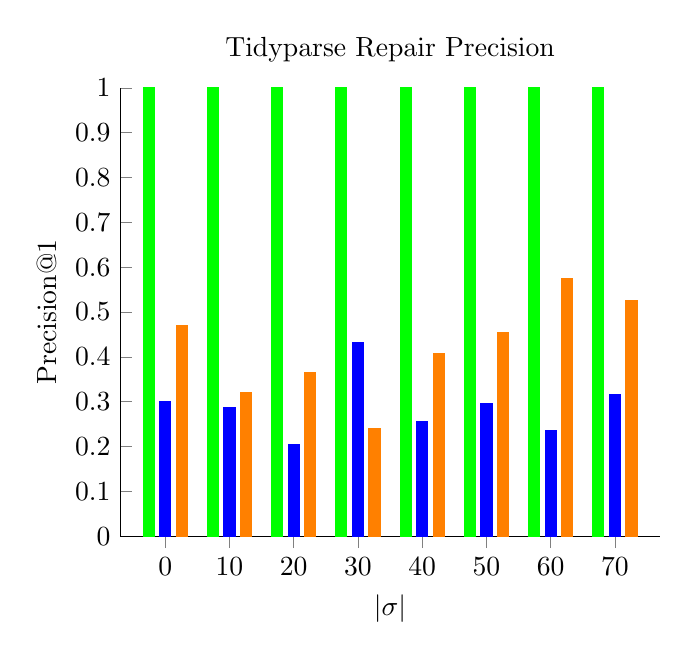
\begin{tikzpicture}
  \begin{axis}[
    xlabel={$|\sigma|$},
    ylabel={Precision@1},
    title={Tidyparse Repair Precision},
    ybar,
    axis lines*=left,
    xtick={0, 10, 20, 30, 40, 50, 60, 70},
    ytick={0, 0.1, 0.2, 0.3, 0.4, 0.5, 0.6, 0.7, 0.8, 0.9, 1.0},
    ymax=1.0,
    ymin=0.0,
    bar width=4pt,
  ]

  \addplot[green, fill=green] coordinates {(0, 1.0) (10, 1.0) (20, 1.0) (30, 1.0) (40, 1.0) (50, 1.0) (60, 1.0) (70, 1.0)};
  \addplot[blue, fill=blue] coordinates {(0, 0.3) (10, 0.286) (20, 0.205) (30, 0.433) (40, 0.256) (50, 0.296) (60, 0.236) (70, 0.315)};
  \addplot[orange, fill=orange] coordinates {(0, 0.46875) (10, 0.321) (20, 0.366) (30, 0.24) (40, 0.407) (50, 0.454) (60, 0.574) (70, 0.526)};

%  \legend{Δ=1,Δ=2,Δ=3}
  \end{axis}
\end{tikzpicture}}
  \resizebox{.24\textwidth}{!}{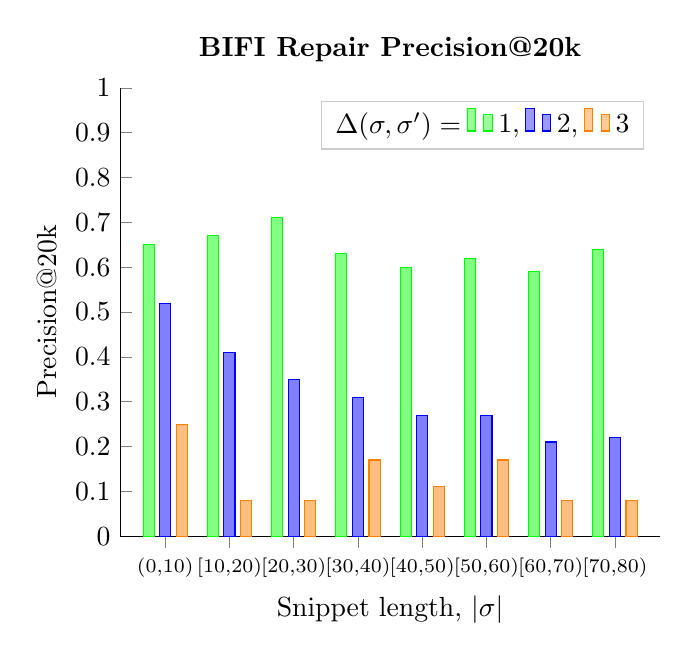
\begin{tikzpicture}
  \begin{axis}[
  xlabel={Snippet length, $|\sigma|$},
  ylabel={Precision@20k},
  title={\textbf{BIFI Repair Precision@20k}},
  legend cell align={left},
  legend style={fill opacity=0.8, draw opacity=1, text opacity=1, draw=lightgray204, legend columns=-1, legend pos=north east},
  ybar,
  axis lines*=left,
  xtick={0, 10, 20, 30, 40, 50, 60, 70},
  ytick={0, 0.1, 0.2, 0.3, 0.4, 0.5, 0.6, 0.7, 0.8, 0.9, 1.0},
  xticklabels={{(}0{,}10{)}, {[}10{,}20{)}, {[}20{,}30{)}, {[}30{,}40{)}, {[}40{,}50{)}, {[}50{,}60{)}, {[}60{,}70{)}, {[}70{,}80{)}},
  x tick label style={font=\scriptsize},
  ymax=1.0,
  ymin=0.0,
  bar width=4pt,
  ]

  \addlegendimage{empty legend}
  \addlegendentry{$\Delta(\err\sigma, \sigma')=$}
  \addlegendimage{ybar,ybar legend,draw=none,green,fill=green!50}
  \addlegendentry{1,}
  \addlegendimage{ybar,ybar legend,draw=none,blue,fill=blue!50}
  \addlegendentry{2,}
  \addlegendimage{ybar,ybar legend,draw=none,orange,fill=orange!50}
  \addlegendentry{3}

  \addplot[green, fill=green!50] coordinates   {(0, 0.65) (10, 0.67) (20, 0.71) (30, 0.63) (40, 0.60) (50, 0.62) (60, 0.59) (70, 0.64)};
  \addplot[blue, fill=blue!50] coordinates     {(0, 0.52) (10, 0.41) (20, 0.35) (30, 0.31) (40, 0.27) (50, 0.27) (60, 0.21) (70, 0.22)};
  \addplot[orange, fill=orange!50] coordinates {(0, 0.25) (10, 0.08) (20, 0.08) (30, 0.17) (40, 0.11) (50, 0.17) (60, 0.08) (70, 0.08)};

  \end{axis}
\end{tikzpicture}
}
  \resizebox{.24\textwidth}{!}{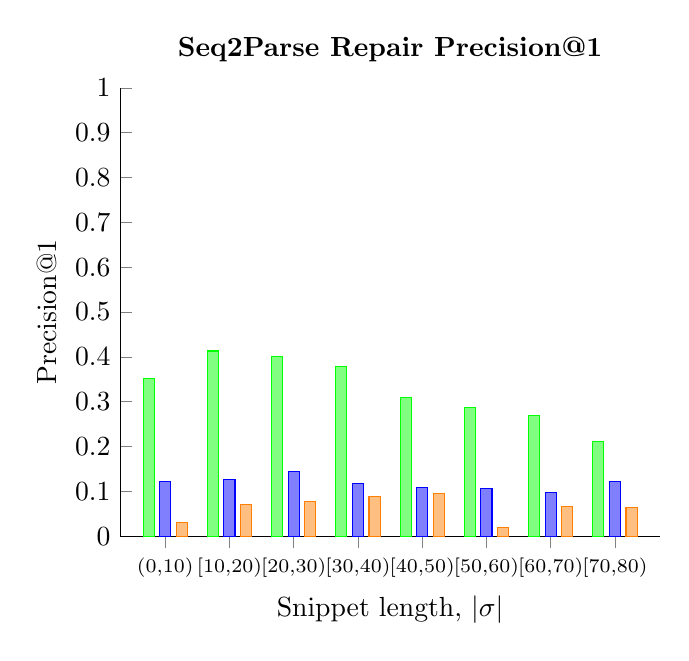
\begin{tikzpicture}
  \begin{axis}[
    xlabel={Snippet length, $|\sigma|$},
    ylabel={Precision@1},
    title={\textbf{Seq2Parse Repair Precision@1}},
    ybar,
    axis lines*=left,
    xtick={0, 10, 20, 30, 40, 50, 60, 70},
    ytick={0, 0.1, 0.2, 0.3, 0.4, 0.5, 0.6, 0.7, 0.8, 0.9, 1.0},
    xticklabels={{(}0{,}10{)}, {[}10{,}20{)}, {[}20{,}30{)}, {[}30{,}40{)}, {[}40{,}50{)}, {[}50{,}60{)}, {[}60{,}70{)}, {[}70{,}80{)}},
    x tick label style={font=\scriptsize},
    ymax=1.0,
    ymin=0.0,
    bar width=4pt,
  ]

  \addplot[green, fill=green!50] coordinates {(0, 0.352631) (10, 0.413115) (20, 0.400502) (30, 0.378440) (40, 0.308869) (50, 0.287755) (60, 0.268817) (70, 0.210526)};
  \addplot[blue, fill=blue!50] coordinates {(0, 0.122529) (10, 0.126453) (20, 0.144192) (30, 0.118483) (40, 0.108007) (50, 0.106849) (60, 0.097403) (70, 0.122047)};
  \addplot[orange, fill=orange!50] coordinates {(0, 0.03125) (10, 0.070922) (20, 0.077348) (30, 0.087629) (40, 0.094675) (50, 0.02) (60, 0.066038) (70, 0.063291)};

  \end{axis}
\end{tikzpicture}}
  \resizebox{.24\textwidth}{!}{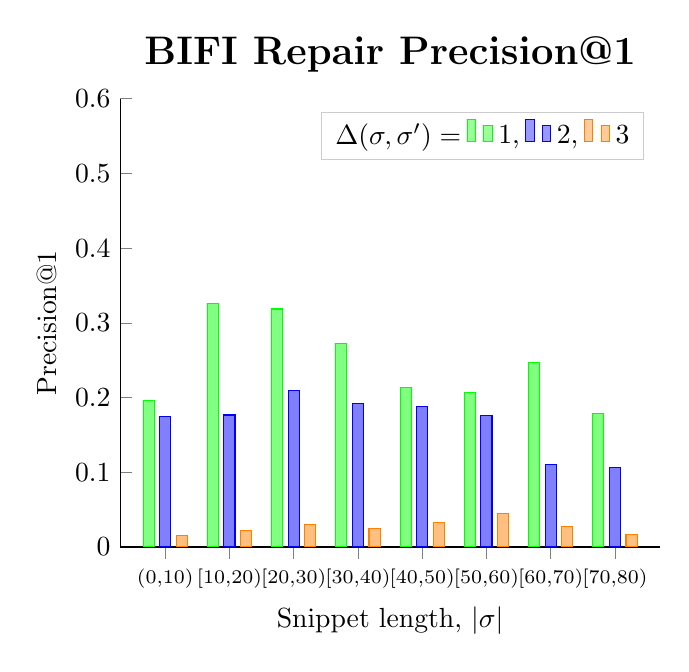
\begin{tikzpicture}
  \begin{axis}[
    legend cell align={left},
    legend style={fill opacity=0.8, draw opacity=1, text opacity=1, draw=lightgray204, legend columns=-1, legend pos=north east},
    xlabel={Snippet length, $|\sigma|$},
    ylabel={Precision@1},
    title={\Large\textbf{BIFI Repair Precision@1}},
    ybar,
    axis lines*=left,
    xtick={0, 10, 20, 30, 40, 50, 60, 70},
    ytick={0, 0.1, 0.2, 0.3, 0.4, 0.5, 0.6, 0.7, 0.8, 0.9, 1.0},
    xticklabels={{(}0{,}10{)}, {[}10{,}20{)}, {[}20{,}30{)}, {[}30{,}40{)}, {[}40{,}50{)}, {[}50{,}60{)}, {[}60{,}70{)}, {[}70{,}80{)}},
    x tick label style={font=\scriptsize},
    ymax=0.6,
    ymin=0.0,
    bar width=4pt,
  ]
    \addlegendimage{empty legend}
    \addlegendentry{$\Delta(\err\sigma, \sigma')=$}
    \addlegendimage{ybar,ybar legend,draw=none,green,fill=green!50}
    \addlegendentry{1,}
    \addlegendimage{ybar,ybar legend,draw=none,blue,fill=blue!50}
    \addlegendentry{2,}
    \addlegendimage{ybar,ybar legend,draw=none,orange,fill=orange!50}
    \addlegendentry{3}

    \addplot[green, fill=green!50] coordinates {(0, 0.196013) (10, 0.326401) (20, 0.318538) (30, 0.272843) (40, 0.213894) (50, 0.206651) (60, 0.247525) (70, 0.179245)};
    \addplot[blue, fill=blue!50] coordinates {(0, 0.174603) (10, 0.176651) (20, 0.209573) (30, 0.19195) (40, 0.18851) (50, 0.176166) (60, 0.110787) (70, 0.106383)};
    \addplot[orange, fill=orange!50] coordinates {(0, 0.015873) (10, 0.021858) (20, 0.030435) (30, 0.02439) (40, 0.032922) (50, 0.045) (60, 0.027397) (70, 0.017094)};
  \end{axis}
\end{tikzpicture}}
  \caption{Tidyparse, Seq2Parse and BIFI repair precision across length and edits.}
\end{figure}

If we give it an equivalent number of samples, the constrained Markov model attains an even wider margin.

\begin{figure}[H]
  \resizebox{.24\textwidth}{!}{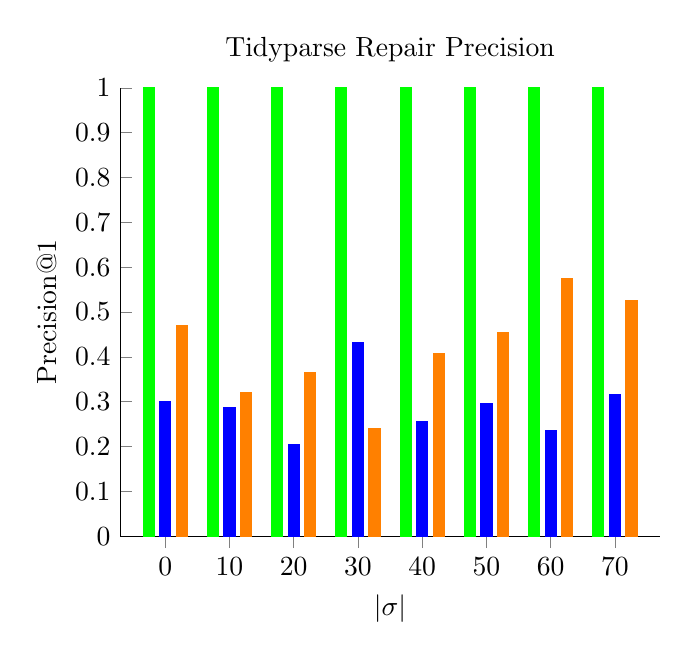
\begin{tikzpicture}
  \begin{axis}[
    xlabel={$|\sigma|$},
    ylabel={Precision@1},
    title={Tidyparse Repair Precision},
    ybar,
    axis lines*=left,
    xtick={0, 10, 20, 30, 40, 50, 60, 70},
    ytick={0, 0.1, 0.2, 0.3, 0.4, 0.5, 0.6, 0.7, 0.8, 0.9, 1.0},
    ymax=1.0,
    ymin=0.0,
    bar width=4pt,
  ]

  \addplot[green, fill=green] coordinates {(0, 1.0) (10, 1.0) (20, 1.0) (30, 1.0) (40, 1.0) (50, 1.0) (60, 1.0) (70, 1.0)};
  \addplot[blue, fill=blue] coordinates {(0, 0.3) (10, 0.286) (20, 0.205) (30, 0.433) (40, 0.256) (50, 0.296) (60, 0.236) (70, 0.315)};
  \addplot[orange, fill=orange] coordinates {(0, 0.46875) (10, 0.321) (20, 0.366) (30, 0.24) (40, 0.407) (50, 0.454) (60, 0.574) (70, 0.526)};

%  \legend{Δ=1,Δ=2,Δ=3}
  \end{axis}
\end{tikzpicture}}
  \resizebox{.24\textwidth}{!}{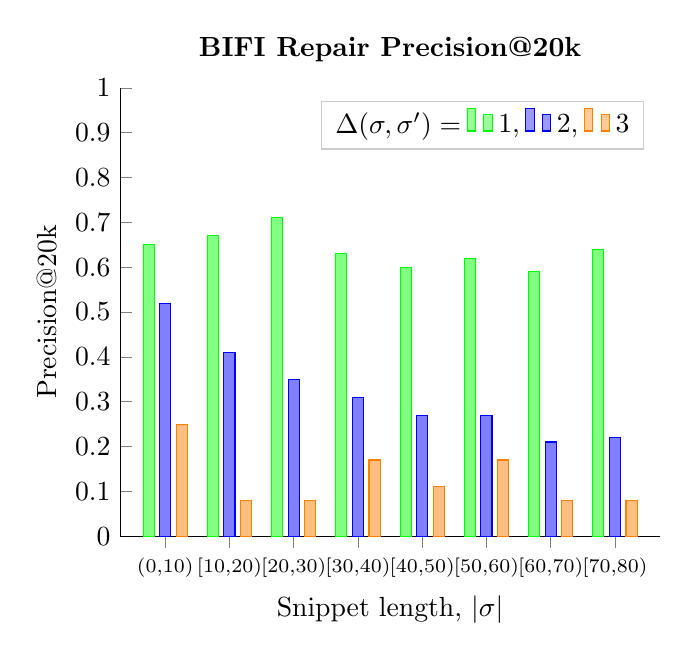
\begin{tikzpicture}
  \begin{axis}[
  xlabel={Snippet length, $|\sigma|$},
  ylabel={Precision@20k},
  title={\textbf{BIFI Repair Precision@20k}},
  legend cell align={left},
  legend style={fill opacity=0.8, draw opacity=1, text opacity=1, draw=lightgray204, legend columns=-1, legend pos=north east},
  ybar,
  axis lines*=left,
  xtick={0, 10, 20, 30, 40, 50, 60, 70},
  ytick={0, 0.1, 0.2, 0.3, 0.4, 0.5, 0.6, 0.7, 0.8, 0.9, 1.0},
  xticklabels={{(}0{,}10{)}, {[}10{,}20{)}, {[}20{,}30{)}, {[}30{,}40{)}, {[}40{,}50{)}, {[}50{,}60{)}, {[}60{,}70{)}, {[}70{,}80{)}},
  x tick label style={font=\scriptsize},
  ymax=1.0,
  ymin=0.0,
  bar width=4pt,
  ]

  \addlegendimage{empty legend}
  \addlegendentry{$\Delta(\err\sigma, \sigma')=$}
  \addlegendimage{ybar,ybar legend,draw=none,green,fill=green!50}
  \addlegendentry{1,}
  \addlegendimage{ybar,ybar legend,draw=none,blue,fill=blue!50}
  \addlegendentry{2,}
  \addlegendimage{ybar,ybar legend,draw=none,orange,fill=orange!50}
  \addlegendentry{3}

  \addplot[green, fill=green!50] coordinates   {(0, 0.65) (10, 0.67) (20, 0.71) (30, 0.63) (40, 0.60) (50, 0.62) (60, 0.59) (70, 0.64)};
  \addplot[blue, fill=blue!50] coordinates     {(0, 0.52) (10, 0.41) (20, 0.35) (30, 0.31) (40, 0.27) (50, 0.27) (60, 0.21) (70, 0.22)};
  \addplot[orange, fill=orange!50] coordinates {(0, 0.25) (10, 0.08) (20, 0.08) (30, 0.17) (40, 0.11) (50, 0.17) (60, 0.08) (70, 0.08)};

  \end{axis}
\end{tikzpicture}
}
  \resizebox{.24\textwidth}{!}{\input{../popl2025/len_dist_tidy200}}
  \resizebox{.24\textwidth}{!}{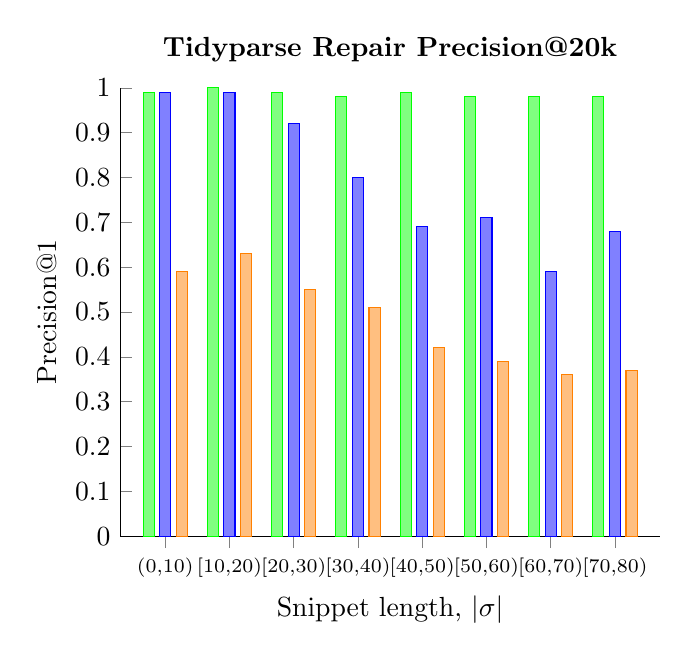
\begin{tikzpicture}
  \begin{axis}[
    xlabel={Snippet length, $|\sigma|$},
    ylabel={Precision@1},
    title={\textbf{Tidyparse Repair Precision@20k}},
    ybar,
    axis lines*=left,
    xtick={0, 10, 20, 30, 40, 50, 60, 70},
    ytick={0, 0.1, 0.2, 0.3, 0.4, 0.5, 0.6, 0.7, 0.8, 0.9, 1.0},
    xticklabels={{(}0{,}10{)}, {[}10{,}20{)}, {[}20{,}30{)}, {[}30{,}40{)}, {[}40{,}50{)}, {[}50{,}60{)}, {[}60{,}70{)}, {[}70{,}80{)}},
    x tick label style={font=\scriptsize},
    ymax=1.0,
    ymin=0.0,
    bar width=4pt,
  ]

  \addplot[green, fill=green!50] coordinates   {(0, 0.99) (10, 1.00) (20, 0.99) (30, 0.98) (40, 0.99) (50, 0.98) (60, 0.98) (70, 0.98)};
  \addplot[blue, fill=blue!50] coordinates     {(0, 0.99) (10, 0.99) (20, 0.92) (30, 0.80) (40, 0.69) (50, 0.71) (60, 0.59) (70, 0.68)};
  \addplot[orange, fill=orange!50] coordinates {(0, 0.59) (10, 0.63) (20, 0.55) (30, 0.51) (40, 0.42) (50, 0.39) (60, 0.36) (70, 0.37)};

  \end{axis}
\end{tikzpicture}

%                                    TIDY-GWA                     TIDY-CFG                  TIDY-ENUM
%(|σ|∈[0, 10), Δ=1): Top-1/total:    56 / 100 = 0.56               54 / 99 = 0.55            57 / 100 = 0.57
%(|σ|∈[0, 10), Δ=2): Top-1/total:    37 / 100 = 0.37              19 / 100 = 0.19            22 / 100 = 0.22
%(|σ|∈[0, 10), Δ=3): Top-1/total:      9 / 50 = 0.18                6 / 50 = 0.12              6 / 50 = 0.12

%(|σ|∈[10, 20), Δ=1): Top-1/total:   44 / 100 = 0.44              42 / 100 = 0.42            45 / 100 = 0.45
%(|σ|∈[10, 20), Δ=2): Top-1/total:   28 / 100 = 0.28              13 / 100 = 0.13            14 / 100 = 0.14
%(|σ|∈[10, 20), Δ=3): Top-1/total:   20 / 100 = 0.20               9 / 100 = 0.09             8 / 100 = 0.08

%(|σ|∈[20, 30), Δ=1): Top-1/total:   43 / 100 = 0.43              49 / 100 = 0.49            49 / 100 = 0.49
%(|σ|∈[20, 30), Δ=2): Top-1/total:   26 / 100 = 0.26              13 / 100 = 0.13            18 / 100 = 0.18
%(|σ|∈[20, 30), Δ=3): Top-1/total:    19 / 99 = 0.19                8 / 99 = 0.08              8 / 99 = 0.08

%(|σ|∈[30, 40), Δ=1): Top-1/total:   49 / 100 = 0.49              43 / 100 = 0.43            48 / 100 = 0.48
%(|σ|∈[30, 40), Δ=2): Top-1/total:   24 / 100 = 0.24              15 / 100 = 0.15            18 / 100 = 0.18
%(|σ|∈[30, 40), Δ=3): Top-1/total:   15 / 100 = 0.15              10 / 100 = 0.10             6 / 100 = 0.06

%(|σ|∈[40, 50), Δ=1): Top-1/total:   55 / 100 = 0.55              56 / 100 = 0.56            57 / 100 = 0.57
%(|σ|∈[40, 50), Δ=2): Top-1/total:   19 / 100 = 0.19              21 / 100 = 0.21            18 / 100 = 0.18
%(|σ|∈[40, 50), Δ=3): Top-1/total:   10 / 100 = 0.10               8 / 100 = 0.08             5 / 100 = 0.05

%(|σ|∈[50, 60), Δ=1): Top-1/total:   55 / 100 = 0.55              67 / 100 = 0.67            53 / 100 = 0.53
%(|σ|∈[50, 60), Δ=2): Top-1/total:   25 / 100 = 0.25              16 / 100 = 0.16            21 / 100 = 0.21
%(|σ|∈[50, 60), Δ=3): Top-1/total:    9 / 100 = 0.09               9 / 100 = 0.09             7 / 100 = 0.07

%(|σ|∈[60, 70), Δ=1): Top-1/total:   53 / 100 = 0.53              56 / 100 = 0.56            60 / 100 = 0.60
%(|σ|∈[60, 70), Δ=2): Top-1/total:   23 / 100 = 0.23              15 / 100 = 0.15            10 / 100 = 0.10
%(|σ|∈[60, 70), Δ=3): Top-1/total:   11 / 100 = 0.11               5 / 100 = 0.05             2 / 100 = 0.02

%(|σ|∈[70, 80), Δ=1): Top-1/total:   57 / 100 = 0.57              62 / 100 = 0.62            63 / 100 = 0.63
%(|σ|∈[70, 80), Δ=2): Top-1/total:   18 / 100 = 0.18              12 / 100 = 0.12            15 / 100 = 0.15
%(|σ|∈[70, 80), Δ=3): Top-1/total:     9 / 81 = 0.11                4 / 81 = 0.05              3 / 81 = 0.04}
  \caption{Tidyparse, Seq2Parse and BIFI repair precision across length and edits.}
\end{figure}

Now, we measure latency.

\begin{figure}[H]
%    \resizebox{.19\textwidth}{!}{% This file was created with tikzplotlib v0.10.1.
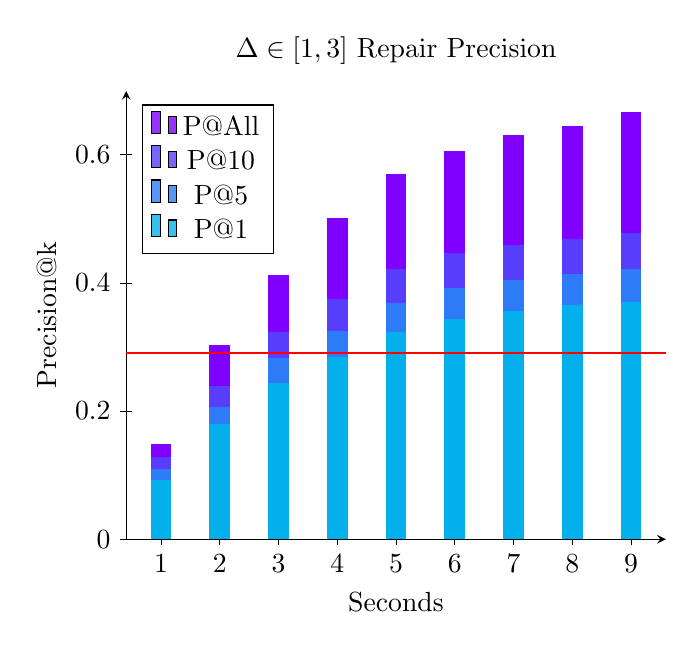
\begin{tikzpicture}

\definecolor{darkgray176}{RGB}{176,176,176}
\definecolor{darkviolet1270255}{RGB}{127,0,255}
\definecolor{deepskyblue3176236}{RGB}{3,176,236}
\definecolor{dodgerblue45123246}{RGB}{45,123,246}
\definecolor{royalblue8762253}{RGB}{87,62,253}

\begin{axis}[
tick align=outside,
tick pos=left,
axis lines=left,
title={\(\displaystyle \Delta\in[1,3]\) Repair Precision},
legend style={fill opacity=0.8, draw opacity=1, text opacity=1, legend columns=1, legend pos=north west},
x grid style={darkgray176},
xlabel={Seconds},
xmin=-0.5925, xmax=8.5925,
xtick style={color=black},
xtick={0,1,2,3,4,5,6,7,8},
xticklabels={1,2,3,4,5,6,7,8,9},
y grid style={darkgray176},
ylabel={Precision@k},
ymin=0, ymax=0.6993,
ytick style={color=black}
]
\draw[draw=none,fill=darkviolet1270255] (axis cs:-0.175,0) rectangle (axis cs:0.175,0.149);
\addlegendimage{ybar,ybar legend,draw=none,fill=darkviolet1270255}
\addlegendentry{P@All}

\draw[draw=none,fill=darkviolet1270255] (axis cs:0.825,0) rectangle (axis cs:1.175,0.303);
\draw[draw=none,fill=darkviolet1270255] (axis cs:1.825,0) rectangle (axis cs:2.175,0.412);
\draw[draw=none,fill=darkviolet1270255] (axis cs:2.825,0) rectangle (axis cs:3.175,0.501);
\draw[draw=none,fill=darkviolet1270255] (axis cs:3.825,0) rectangle (axis cs:4.175,0.569);
\draw[draw=none,fill=darkviolet1270255] (axis cs:4.825,0) rectangle (axis cs:5.175,0.605);
\draw[draw=none,fill=darkviolet1270255] (axis cs:5.825,0) rectangle (axis cs:6.175,0.63);
\draw[draw=none,fill=darkviolet1270255] (axis cs:6.825,0) rectangle (axis cs:7.175,0.645);
\draw[draw=none,fill=darkviolet1270255] (axis cs:7.825,0) rectangle (axis cs:8.175,0.666);
\draw[draw=none,fill=royalblue8762253] (axis cs:-0.175,0) rectangle (axis cs:0.175,0.128);
\addlegendimage{ybar,ybar legend,draw=none,fill=royalblue8762253}
\addlegendentry{P@10}

\draw[draw=none,fill=royalblue8762253] (axis cs:0.825,0) rectangle (axis cs:1.175,0.239);
\draw[draw=none,fill=royalblue8762253] (axis cs:1.825,0) rectangle (axis cs:2.175,0.323);
\draw[draw=none,fill=royalblue8762253] (axis cs:2.825,0) rectangle (axis cs:3.175,0.374);
\draw[draw=none,fill=royalblue8762253] (axis cs:3.825,0) rectangle (axis cs:4.175,0.421);
\draw[draw=none,fill=royalblue8762253] (axis cs:4.825,0) rectangle (axis cs:5.175,0.446);
\draw[draw=none,fill=royalblue8762253] (axis cs:5.825,0) rectangle (axis cs:6.175,0.459);
\draw[draw=none,fill=royalblue8762253] (axis cs:6.825,0) rectangle (axis cs:7.175,0.469);
\draw[draw=none,fill=royalblue8762253] (axis cs:7.825,0) rectangle (axis cs:8.175,0.477);
\draw[draw=none,fill=dodgerblue45123246] (axis cs:-0.175,0) rectangle (axis cs:0.175,0.11);
\addlegendimage{ybar,ybar legend,draw=none,fill=dodgerblue45123246}
\addlegendentry{P@5}

\draw[draw=none,fill=dodgerblue45123246] (axis cs:0.825,0) rectangle (axis cs:1.175,0.206);
\draw[draw=none,fill=dodgerblue45123246] (axis cs:1.825,0) rectangle (axis cs:2.175,0.282);
\draw[draw=none,fill=dodgerblue45123246] (axis cs:2.825,0) rectangle (axis cs:3.175,0.325);
\draw[draw=none,fill=dodgerblue45123246] (axis cs:3.825,0) rectangle (axis cs:4.175,0.369);
\draw[draw=none,fill=dodgerblue45123246] (axis cs:4.825,0) rectangle (axis cs:5.175,0.392);
\draw[draw=none,fill=dodgerblue45123246] (axis cs:5.825,0) rectangle (axis cs:6.175,0.405);
\draw[draw=none,fill=dodgerblue45123246] (axis cs:6.825,0) rectangle (axis cs:7.175,0.414);
\draw[draw=none,fill=dodgerblue45123246] (axis cs:7.825,0) rectangle (axis cs:8.175,0.422);
\draw[draw=none,fill=deepskyblue3176236] (axis cs:-0.175,0) rectangle (axis cs:0.175,0.092);
\addlegendimage{ybar,ybar legend,draw=none,fill=deepskyblue3176236}
\addlegendentry{P@1}

\draw[draw=none,fill=deepskyblue3176236] (axis cs:0.825,0) rectangle (axis cs:1.175,0.18);
\draw[draw=none,fill=deepskyblue3176236] (axis cs:1.825,0) rectangle (axis cs:2.175,0.244);
\draw[draw=none,fill=deepskyblue3176236] (axis cs:2.825,0) rectangle (axis cs:3.175,0.285);
\draw[draw=none,fill=deepskyblue3176236] (axis cs:3.825,0) rectangle (axis cs:4.175,0.324);
\draw[draw=none,fill=deepskyblue3176236] (axis cs:4.825,0) rectangle (axis cs:5.175,0.343);
\draw[draw=none,fill=deepskyblue3176236] (axis cs:5.825,0) rectangle (axis cs:6.175,0.356);
\draw[draw=none,fill=deepskyblue3176236] (axis cs:6.825,0) rectangle (axis cs:7.175,0.365);
\draw[draw=none,fill=deepskyblue3176236] (axis cs:7.825,0) rectangle (axis cs:8.175,0.37);
\addplot [red, thick] coordinates {(-0.8925,0.29) (14.8925,0.29)};
\end{axis}

\end{tikzpicture}
}
  \resizebox{.24\textwidth}{!}{% This file was created with tikzplotlib v0.10.1.
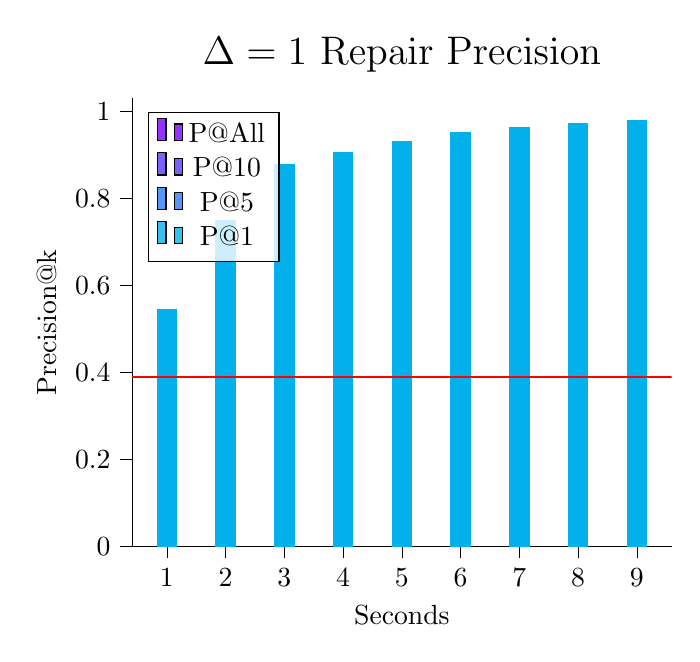
\begin{tikzpicture}

\definecolor{darkgray176}{RGB}{176,176,176}
\definecolor{darkviolet1270255}{RGB}{127,0,255}
\definecolor{deepskyblue3176236}{RGB}{3,176,236}
\definecolor{dodgerblue45123246}{RGB}{45,123,246}
\definecolor{royalblue8762253}{RGB}{87,62,253}

\begin{axis}[
tick align=outside,
tick pos=left,
axis lines*=left,
title={{\Large\(\displaystyle \Delta=1\) Repair Precision}},
legend style={fill opacity=0.8, draw opacity=1, text opacity=1, legend columns=1, legend pos=north west},
x grid style={darkgray176},
xlabel={Seconds},
xmin=-0.5925, xmax=8.5925,
xtick style={color=black},
xtick={0,1,2,3,4,5,6,7,8},
xticklabels={1,2,3,4,5,6,7,8,9},
y grid style={darkgray176},
ylabel={Precision@k},
ymin=0, ymax=1.0311,
ytick style={color=black}
]
\draw[draw=none,fill=darkviolet1270255] (axis cs:-0.175,0) rectangle (axis cs:0.175,0.546);
\addlegendimage{ybar,ybar legend,draw=none,fill=darkviolet1270255}
\addlegendentry{P@All}

\draw[draw=none,fill=darkviolet1270255] (axis cs:0.825,0) rectangle (axis cs:1.175,0.752);
\draw[draw=none,fill=darkviolet1270255] (axis cs:1.825,0) rectangle (axis cs:2.175,0.88);
\draw[draw=none,fill=darkviolet1270255] (axis cs:2.825,0) rectangle (axis cs:3.175,0.908);
\draw[draw=none,fill=darkviolet1270255] (axis cs:3.825,0) rectangle (axis cs:4.175,0.933);
\draw[draw=none,fill=darkviolet1270255] (axis cs:4.825,0) rectangle (axis cs:5.175,0.954);
\draw[draw=none,fill=darkviolet1270255] (axis cs:5.825,0) rectangle (axis cs:6.175,0.966);
\draw[draw=none,fill=darkviolet1270255] (axis cs:6.825,0) rectangle (axis cs:7.175,0.975);
\draw[draw=none,fill=darkviolet1270255] (axis cs:7.825,0) rectangle (axis cs:8.175,0.982);
\draw[draw=none,fill=royalblue8762253] (axis cs:-0.175,0) rectangle (axis cs:0.175,0.546);
\addlegendimage{ybar,ybar legend,draw=none,fill=royalblue8762253}
\addlegendentry{P@10}

\draw[draw=none,fill=royalblue8762253] (axis cs:0.825,0) rectangle (axis cs:1.175,0.752);
\draw[draw=none,fill=royalblue8762253] (axis cs:1.825,0) rectangle (axis cs:2.175,0.88);
\draw[draw=none,fill=royalblue8762253] (axis cs:2.825,0) rectangle (axis cs:3.175,0.908);
\draw[draw=none,fill=royalblue8762253] (axis cs:3.825,0) rectangle (axis cs:4.175,0.933);
\draw[draw=none,fill=royalblue8762253] (axis cs:4.825,0) rectangle (axis cs:5.175,0.954);
\draw[draw=none,fill=royalblue8762253] (axis cs:5.825,0) rectangle (axis cs:6.175,0.966);
\draw[draw=none,fill=royalblue8762253] (axis cs:6.825,0) rectangle (axis cs:7.175,0.975);
\draw[draw=none,fill=royalblue8762253] (axis cs:7.825,0) rectangle (axis cs:8.175,0.982);
\draw[draw=none,fill=dodgerblue45123246] (axis cs:-0.175,0) rectangle (axis cs:0.175,0.546);
\addlegendimage{ybar,ybar legend,draw=none,fill=dodgerblue45123246}
\addlegendentry{P@5}

\draw[draw=none,fill=dodgerblue45123246] (axis cs:0.825,0) rectangle (axis cs:1.175,0.752);
\draw[draw=none,fill=dodgerblue45123246] (axis cs:1.825,0) rectangle (axis cs:2.175,0.88);
\draw[draw=none,fill=dodgerblue45123246] (axis cs:2.825,0) rectangle (axis cs:3.175,0.908);
\draw[draw=none,fill=dodgerblue45123246] (axis cs:3.825,0) rectangle (axis cs:4.175,0.933);
\draw[draw=none,fill=dodgerblue45123246] (axis cs:4.825,0) rectangle (axis cs:5.175,0.954);
\draw[draw=none,fill=dodgerblue45123246] (axis cs:5.825,0) rectangle (axis cs:6.175,0.966);
\draw[draw=none,fill=dodgerblue45123246] (axis cs:6.825,0) rectangle (axis cs:7.175,0.975);
\draw[draw=none,fill=dodgerblue45123246] (axis cs:7.825,0) rectangle (axis cs:8.175,0.982);
\draw[draw=none,fill=deepskyblue3176236] (axis cs:-0.175,0) rectangle (axis cs:0.175,0.546);
\addlegendimage{ybar,ybar legend,draw=none,fill=deepskyblue3176236}
\addlegendentry{P@1}

\draw[draw=none,fill=deepskyblue3176236] (axis cs:0.825,0) rectangle (axis cs:1.175,0.752);
\draw[draw=none,fill=deepskyblue3176236] (axis cs:1.825,0) rectangle (axis cs:2.175,0.88);
\draw[draw=none,fill=deepskyblue3176236] (axis cs:2.825,0) rectangle (axis cs:3.175,0.908);
\draw[draw=none,fill=deepskyblue3176236] (axis cs:3.825,0) rectangle (axis cs:4.175,0.933);
\draw[draw=none,fill=deepskyblue3176236] (axis cs:4.825,0) rectangle (axis cs:5.175,0.954);
\draw[draw=none,fill=deepskyblue3176236] (axis cs:5.825,0) rectangle (axis cs:6.175,0.966);
\draw[draw=none,fill=deepskyblue3176236] (axis cs:6.825,0) rectangle (axis cs:7.175,0.975);
\draw[draw=none,fill=deepskyblue3176236] (axis cs:7.825,0) rectangle (axis cs:8.175,0.982);
\addplot [red, thick] coordinates {(-0.8925,0.39) (14.8925,0.39)};
\end{axis}

\end{tikzpicture}
}
  \resizebox{.24\textwidth}{!}{% This file was created with tikzplotlib v0.10.1.
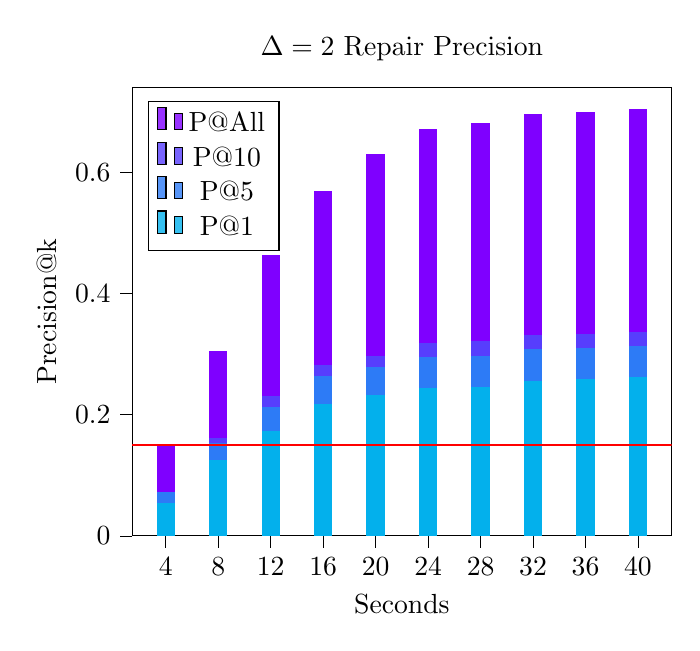
\begin{tikzpicture}

\definecolor{darkgray176}{RGB}{176,176,176}
\definecolor{darkviolet1270255}{RGB}{127,0,255}
\definecolor{deepskyblue3176236}{RGB}{3,176,236}
\definecolor{dodgerblue45123246}{RGB}{45,123,246}
\definecolor{royalblue8762253}{RGB}{87,62,253}

\begin{axis}[
tick align=outside,
tick pos=left,
title={\(\displaystyle \Delta=2\) Repair Precision},
legend style={fill opacity=0.8, draw opacity=1, text opacity=1, legend columns=1, legend pos=north west},
x grid style={darkgray176},
xlabel={Seconds},
xmin=-0.6425, xmax=9.6425,
xtick style={color=black},
xtick={0,1,2,3,4,5,6,7,8,9},
xticklabels={4,8,12,16,20,24,28,32,36,40},
y grid style={darkgray176},
ylabel={Precision@k},
ymin=0, ymax=0.74025,
ytick style={color=black}
]
\draw[draw=none,fill=darkviolet1270255] (axis cs:-0.175,0) rectangle (axis cs:0.175,0.149);
\addlegendimage{ybar,ybar legend,draw=none,fill=darkviolet1270255}
\addlegendentry{P@All}

\draw[draw=none,fill=darkviolet1270255] (axis cs:0.825,0) rectangle (axis cs:1.175,0.305);
\draw[draw=none,fill=darkviolet1270255] (axis cs:1.825,0) rectangle (axis cs:2.175,0.464);
\draw[draw=none,fill=darkviolet1270255] (axis cs:2.825,0) rectangle (axis cs:3.175,0.569);
\draw[draw=none,fill=darkviolet1270255] (axis cs:3.825,0) rectangle (axis cs:4.175,0.631);
\draw[draw=none,fill=darkviolet1270255] (axis cs:4.825,0) rectangle (axis cs:5.175,0.672);
\draw[draw=none,fill=darkviolet1270255] (axis cs:5.825,0) rectangle (axis cs:6.175,0.682);
\draw[draw=none,fill=darkviolet1270255] (axis cs:6.825,0) rectangle (axis cs:7.175,0.697);
\draw[draw=none,fill=darkviolet1270255] (axis cs:7.825,0) rectangle (axis cs:8.175,0.7);
\draw[draw=none,fill=darkviolet1270255] (axis cs:8.825,0) rectangle (axis cs:9.175,0.705);
\draw[draw=none,fill=royalblue8762253] (axis cs:-0.175,0) rectangle (axis cs:0.175,0.072);
\addlegendimage{ybar,ybar legend,draw=none,fill=royalblue8762253}
\addlegendentry{P@10}

\draw[draw=none,fill=royalblue8762253] (axis cs:0.825,0) rectangle (axis cs:1.175,0.162);
\draw[draw=none,fill=royalblue8762253] (axis cs:1.825,0) rectangle (axis cs:2.175,0.231);
\draw[draw=none,fill=royalblue8762253] (axis cs:2.825,0) rectangle (axis cs:3.175,0.282);
\draw[draw=none,fill=royalblue8762253] (axis cs:3.825,0) rectangle (axis cs:4.175,0.297);
\draw[draw=none,fill=royalblue8762253] (axis cs:4.825,0) rectangle (axis cs:5.175,0.318);
\draw[draw=none,fill=royalblue8762253] (axis cs:5.825,0) rectangle (axis cs:6.175,0.321);
\draw[draw=none,fill=royalblue8762253] (axis cs:6.825,0) rectangle (axis cs:7.175,0.331);
\draw[draw=none,fill=royalblue8762253] (axis cs:7.825,0) rectangle (axis cs:8.175,0.333);
\draw[draw=none,fill=royalblue8762253] (axis cs:8.825,0) rectangle (axis cs:9.175,0.336);
\draw[draw=none,fill=dodgerblue45123246] (axis cs:-0.175,0) rectangle (axis cs:0.175,0.072);
\addlegendimage{ybar,ybar legend,draw=none,fill=dodgerblue45123246}
\addlegendentry{P@5}

\draw[draw=none,fill=dodgerblue45123246] (axis cs:0.825,0) rectangle (axis cs:1.175,0.154);
\draw[draw=none,fill=dodgerblue45123246] (axis cs:1.825,0) rectangle (axis cs:2.175,0.213);
\draw[draw=none,fill=dodgerblue45123246] (axis cs:2.825,0) rectangle (axis cs:3.175,0.264);
\draw[draw=none,fill=dodgerblue45123246] (axis cs:3.825,0) rectangle (axis cs:4.175,0.279);
\draw[draw=none,fill=dodgerblue45123246] (axis cs:4.825,0) rectangle (axis cs:5.175,0.295);
\draw[draw=none,fill=dodgerblue45123246] (axis cs:5.825,0) rectangle (axis cs:6.175,0.297);
\draw[draw=none,fill=dodgerblue45123246] (axis cs:6.825,0) rectangle (axis cs:7.175,0.308);
\draw[draw=none,fill=dodgerblue45123246] (axis cs:7.825,0) rectangle (axis cs:8.175,0.31);
\draw[draw=none,fill=dodgerblue45123246] (axis cs:8.825,0) rectangle (axis cs:9.175,0.313);
\draw[draw=none,fill=deepskyblue3176236] (axis cs:-0.175,0) rectangle (axis cs:0.175,0.054);
\addlegendimage{ybar,ybar legend,draw=none,fill=deepskyblue3176236}
\addlegendentry{P@1}

\draw[draw=none,fill=deepskyblue3176236] (axis cs:0.825,0) rectangle (axis cs:1.175,0.126);
\draw[draw=none,fill=deepskyblue3176236] (axis cs:1.825,0) rectangle (axis cs:2.175,0.174);
\draw[draw=none,fill=deepskyblue3176236] (axis cs:2.825,0) rectangle (axis cs:3.175,0.218);
\draw[draw=none,fill=deepskyblue3176236] (axis cs:3.825,0) rectangle (axis cs:4.175,0.233);
\draw[draw=none,fill=deepskyblue3176236] (axis cs:4.825,0) rectangle (axis cs:5.175,0.244);
\draw[draw=none,fill=deepskyblue3176236] (axis cs:5.825,0) rectangle (axis cs:6.175,0.246);
\draw[draw=none,fill=deepskyblue3176236] (axis cs:6.825,0) rectangle (axis cs:7.175,0.256);
\draw[draw=none,fill=deepskyblue3176236] (axis cs:7.825,0) rectangle (axis cs:8.175,0.259);
\draw[draw=none,fill=deepskyblue3176236] (axis cs:8.825,0) rectangle (axis cs:9.175,0.262);
\addplot [red, thick] coordinates {(-0.8925,0.15) (14.8925,0.15)};
\end{axis}

\end{tikzpicture}
}
  \resizebox{.24\textwidth}{!}{% This file was created with tikzplotlib v0.10.1.
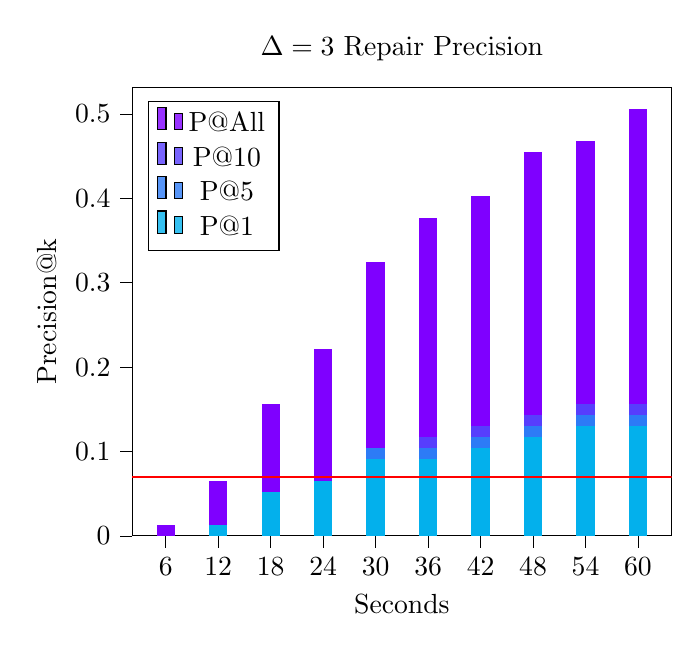
\begin{tikzpicture}

\definecolor{darkgray176}{RGB}{176,176,176}
\definecolor{darkviolet1270255}{RGB}{127,0,255}
\definecolor{deepskyblue3176236}{RGB}{3,176,236}
\definecolor{dodgerblue45123246}{RGB}{45,123,246}
\definecolor{royalblue8762253}{RGB}{87,62,253}

\begin{axis}[
tick align=outside,
tick pos=left,
title={\(\displaystyle \Delta=3\) Repair Precision},
legend style={fill opacity=0.8, draw opacity=1, text opacity=1, legend columns=1, legend pos=north west},
x grid style={darkgray176},
xlabel={Seconds},
xmin=-0.6425, xmax=9.6425,
xtick style={color=black},
xtick={0,1,2,3,4,5,6,7,8,9},
xticklabels={6,12,18,24,30,36,42,48,54,60},
y grid style={darkgray176},
ylabel={Precision@k},
ymin=0, ymax=0.5313,
ytick style={color=black}
]
\draw[draw=none,fill=darkviolet1270255] (axis cs:-0.175,0) rectangle (axis cs:0.175,0.013);
\addlegendimage{ybar,ybar legend,draw=none,fill=darkviolet1270255}
\addlegendentry{P@All}

\draw[draw=none,fill=darkviolet1270255] (axis cs:0.825,0) rectangle (axis cs:1.175,0.065);
\draw[draw=none,fill=darkviolet1270255] (axis cs:1.825,0) rectangle (axis cs:2.175,0.156);
\draw[draw=none,fill=darkviolet1270255] (axis cs:2.825,0) rectangle (axis cs:3.175,0.221);
\draw[draw=none,fill=darkviolet1270255] (axis cs:3.825,0) rectangle (axis cs:4.175,0.325);
\draw[draw=none,fill=darkviolet1270255] (axis cs:4.825,0) rectangle (axis cs:5.175,0.377);
\draw[draw=none,fill=darkviolet1270255] (axis cs:5.825,0) rectangle (axis cs:6.175,0.403);
\draw[draw=none,fill=darkviolet1270255] (axis cs:6.825,0) rectangle (axis cs:7.175,0.455);
\draw[draw=none,fill=darkviolet1270255] (axis cs:7.825,0) rectangle (axis cs:8.175,0.468);
\draw[draw=none,fill=darkviolet1270255] (axis cs:8.825,0) rectangle (axis cs:9.175,0.506);
\draw[draw=none,fill=royalblue8762253] (axis cs:-0.175,0) rectangle (axis cs:0.175,0);
\addlegendimage{ybar,ybar legend,draw=none,fill=royalblue8762253}
\addlegendentry{P@10}

\draw[draw=none,fill=royalblue8762253] (axis cs:0.825,0) rectangle (axis cs:1.175,0.013);
\draw[draw=none,fill=royalblue8762253] (axis cs:1.825,0) rectangle (axis cs:2.175,0.052);
\draw[draw=none,fill=royalblue8762253] (axis cs:2.825,0) rectangle (axis cs:3.175,0.065);
\draw[draw=none,fill=royalblue8762253] (axis cs:3.825,0) rectangle (axis cs:4.175,0.104);
\draw[draw=none,fill=royalblue8762253] (axis cs:4.825,0) rectangle (axis cs:5.175,0.117);
\draw[draw=none,fill=royalblue8762253] (axis cs:5.825,0) rectangle (axis cs:6.175,0.13);
\draw[draw=none,fill=royalblue8762253] (axis cs:6.825,0) rectangle (axis cs:7.175,0.143);
\draw[draw=none,fill=royalblue8762253] (axis cs:7.825,0) rectangle (axis cs:8.175,0.156);
\draw[draw=none,fill=royalblue8762253] (axis cs:8.825,0) rectangle (axis cs:9.175,0.156);
\draw[draw=none,fill=dodgerblue45123246] (axis cs:-0.175,0) rectangle (axis cs:0.175,0);
\addlegendimage{ybar,ybar legend,draw=none,fill=dodgerblue45123246}
\addlegendentry{P@5}

\draw[draw=none,fill=dodgerblue45123246] (axis cs:0.825,0) rectangle (axis cs:1.175,0.013);
\draw[draw=none,fill=dodgerblue45123246] (axis cs:1.825,0) rectangle (axis cs:2.175,0.052);
\draw[draw=none,fill=dodgerblue45123246] (axis cs:2.825,0) rectangle (axis cs:3.175,0.065);
\draw[draw=none,fill=dodgerblue45123246] (axis cs:3.825,0) rectangle (axis cs:4.175,0.104);
\draw[draw=none,fill=dodgerblue45123246] (axis cs:4.825,0) rectangle (axis cs:5.175,0.104);
\draw[draw=none,fill=dodgerblue45123246] (axis cs:5.825,0) rectangle (axis cs:6.175,0.117);
\draw[draw=none,fill=dodgerblue45123246] (axis cs:6.825,0) rectangle (axis cs:7.175,0.13);
\draw[draw=none,fill=dodgerblue45123246] (axis cs:7.825,0) rectangle (axis cs:8.175,0.143);
\draw[draw=none,fill=dodgerblue45123246] (axis cs:8.825,0) rectangle (axis cs:9.175,0.143);
\draw[draw=none,fill=deepskyblue3176236] (axis cs:-0.175,0) rectangle (axis cs:0.175,0);
\addlegendimage{ybar,ybar legend,draw=none,fill=deepskyblue3176236}
\addlegendentry{P@1}

\draw[draw=none,fill=deepskyblue3176236] (axis cs:0.825,0) rectangle (axis cs:1.175,0.013);
\draw[draw=none,fill=deepskyblue3176236] (axis cs:1.825,0) rectangle (axis cs:2.175,0.052);
\draw[draw=none,fill=deepskyblue3176236] (axis cs:2.825,0) rectangle (axis cs:3.175,0.065);
\draw[draw=none,fill=deepskyblue3176236] (axis cs:3.825,0) rectangle (axis cs:4.175,0.091);
\draw[draw=none,fill=deepskyblue3176236] (axis cs:4.825,0) rectangle (axis cs:5.175,0.091);
\draw[draw=none,fill=deepskyblue3176236] (axis cs:5.825,0) rectangle (axis cs:6.175,0.104);
\draw[draw=none,fill=deepskyblue3176236] (axis cs:6.825,0) rectangle (axis cs:7.175,0.117);
\draw[draw=none,fill=deepskyblue3176236] (axis cs:7.825,0) rectangle (axis cs:8.175,0.13);
\draw[draw=none,fill=deepskyblue3176236] (axis cs:8.825,0) rectangle (axis cs:9.175,0.13);
\addplot [red, thick] coordinates {(-0.8925,0.07) (14.8925,0.07)};
\end{axis}

\end{tikzpicture}
}
%    \resizebox{.24\textwidth}{!}{% This file was created with tikzplotlib v0.10.1.
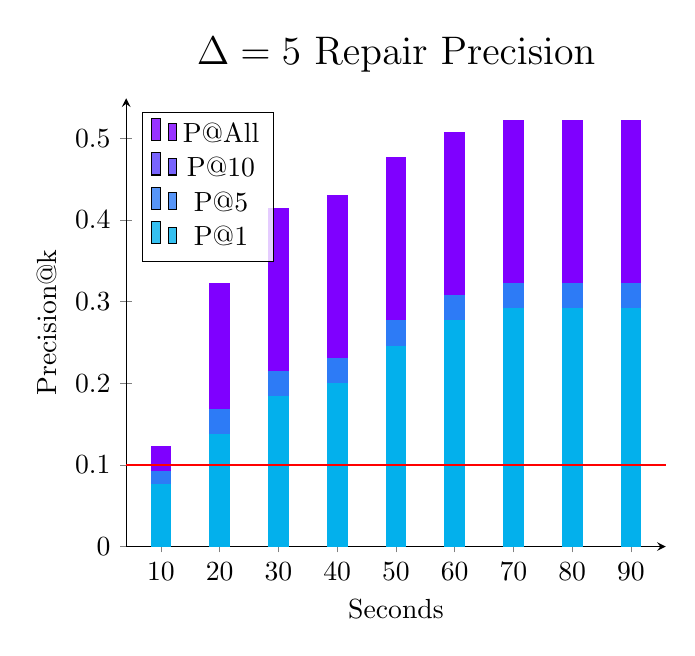
\begin{tikzpicture}
\begin{axis}[
tick align=outside,
tick pos=left,
axis lines=left,
title={\Large\(\displaystyle \Delta=5\) Repair Precision},
legend style={fill opacity=0.8, draw opacity=1, text opacity=1, legend columns=1, legend pos=north west},
x grid style={darkgray176},
xlabel={Seconds},
xmin=-0.5925, xmax=8.5925,
xtick={0,1,2,3,4,5,6,7,8},
xticklabels={10,20,30,40,50,60,70,80,90},
y grid style={darkgray176},
ylabel={Precision@k},
ymin=0, ymax=0.54915,
]
\draw[draw=none,fill=darkviolet1270255] (axis cs:-0.175,0) rectangle (axis cs:0.175,0.123);
\addlegendimage{ybar,ybar legend,draw=none,fill=darkviolet1270255}
\addlegendentry{P@All}

\draw[draw=none,fill=darkviolet1270255] (axis cs:0.825,0) rectangle (axis cs:1.175,0.323);
\draw[draw=none,fill=darkviolet1270255] (axis cs:1.825,0) rectangle (axis cs:2.175,0.415);
\draw[draw=none,fill=darkviolet1270255] (axis cs:2.825,0) rectangle (axis cs:3.175,0.431);
\draw[draw=none,fill=darkviolet1270255] (axis cs:3.825,0) rectangle (axis cs:4.175,0.477);
\draw[draw=none,fill=darkviolet1270255] (axis cs:4.825,0) rectangle (axis cs:5.175,0.508);
\draw[draw=none,fill=darkviolet1270255] (axis cs:5.825,0) rectangle (axis cs:6.175,0.523);
\draw[draw=none,fill=darkviolet1270255] (axis cs:6.825,0) rectangle (axis cs:7.175,0.523);
\draw[draw=none,fill=darkviolet1270255] (axis cs:7.825,0) rectangle (axis cs:8.175,0.523);
\draw[draw=none,fill=royalblue8762253] (axis cs:-0.175,0) rectangle (axis cs:0.175,0.092);
\addlegendimage{ybar,ybar legend,draw=none,fill=royalblue8762253}
\addlegendentry{P@10}

\draw[draw=none,fill=royalblue8762253] (axis cs:0.825,0) rectangle (axis cs:1.175,0.169);
\draw[draw=none,fill=royalblue8762253] (axis cs:1.825,0) rectangle (axis cs:2.175,0.215);
\draw[draw=none,fill=royalblue8762253] (axis cs:2.825,0) rectangle (axis cs:3.175,0.231);
\draw[draw=none,fill=royalblue8762253] (axis cs:3.825,0) rectangle (axis cs:4.175,0.277);
\draw[draw=none,fill=royalblue8762253] (axis cs:4.825,0) rectangle (axis cs:5.175,0.308);
\draw[draw=none,fill=royalblue8762253] (axis cs:5.825,0) rectangle (axis cs:6.175,0.323);
\draw[draw=none,fill=royalblue8762253] (axis cs:6.825,0) rectangle (axis cs:7.175,0.323);
\draw[draw=none,fill=royalblue8762253] (axis cs:7.825,0) rectangle (axis cs:8.175,0.323);
\draw[draw=none,fill=dodgerblue45123246] (axis cs:-0.175,0) rectangle (axis cs:0.175,0.092);
\addlegendimage{ybar,ybar legend,draw=none,fill=dodgerblue45123246}
\addlegendentry{P@5}

\draw[draw=none,fill=dodgerblue45123246] (axis cs:0.825,0) rectangle (axis cs:1.175,0.169);
\draw[draw=none,fill=dodgerblue45123246] (axis cs:1.825,0) rectangle (axis cs:2.175,0.215);
\draw[draw=none,fill=dodgerblue45123246] (axis cs:2.825,0) rectangle (axis cs:3.175,0.231);
\draw[draw=none,fill=dodgerblue45123246] (axis cs:3.825,0) rectangle (axis cs:4.175,0.277);
\draw[draw=none,fill=dodgerblue45123246] (axis cs:4.825,0) rectangle (axis cs:5.175,0.308);
\draw[draw=none,fill=dodgerblue45123246] (axis cs:5.825,0) rectangle (axis cs:6.175,0.323);
\draw[draw=none,fill=dodgerblue45123246] (axis cs:6.825,0) rectangle (axis cs:7.175,0.323);
\draw[draw=none,fill=dodgerblue45123246] (axis cs:7.825,0) rectangle (axis cs:8.175,0.323);
\draw[draw=none,fill=deepskyblue3176236] (axis cs:-0.175,0) rectangle (axis cs:0.175,0.077);
\addlegendimage{ybar,ybar legend,draw=none,fill=deepskyblue3176236}
\addlegendentry{P@1}

\draw[draw=none,fill=deepskyblue3176236] (axis cs:0.825,0) rectangle (axis cs:1.175,0.138);
\draw[draw=none,fill=deepskyblue3176236] (axis cs:1.825,0) rectangle (axis cs:2.175,0.185);
\draw[draw=none,fill=deepskyblue3176236] (axis cs:2.825,0) rectangle (axis cs:3.175,0.2);
\draw[draw=none,fill=deepskyblue3176236] (axis cs:3.825,0) rectangle (axis cs:4.175,0.246);
\draw[draw=none,fill=deepskyblue3176236] (axis cs:4.825,0) rectangle (axis cs:5.175,0.277);
\draw[draw=none,fill=deepskyblue3176236] (axis cs:5.825,0) rectangle (axis cs:6.175,0.292);
\draw[draw=none,fill=deepskyblue3176236] (axis cs:6.825,0) rectangle (axis cs:7.175,0.292);
\draw[draw=none,fill=deepskyblue3176236] (axis cs:7.825,0) rectangle (axis cs:8.175,0.292);
\addplot [red, thick] coordinates {(-0.8925,0.10) (14.8925,0.10)};
\end{axis}

\end{tikzpicture}
}
%\resizebox{.3\textwidth}{!}{% This file was created with tikzplotlib v0.10.1.
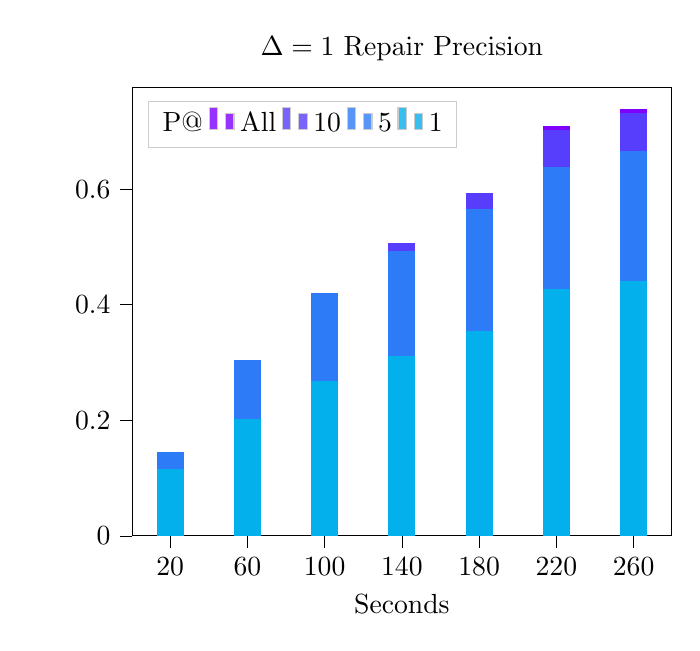
\begin{tikzpicture}

\definecolor{darkgray176}{RGB}{176,176,176}
\definecolor{darkviolet1270255}{RGB}{127,0,255}
\definecolor{deepskyblue3176236}{RGB}{3,176,236}
\definecolor{dodgerblue45123246}{RGB}{45,123,246}
\definecolor{lightgray204}{RGB}{204,204,204}
\definecolor{royalblue8762253}{RGB}{87,62,253}

\begin{axis}[
legend cell align={left},
legend style={fill opacity=0.8, draw opacity=1, text opacity=1, draw=lightgray204, legend columns=-1, legend pos=north west},
tick align=outside,
tick pos=left,
title={$\Delta=1$ Repair Precision},
x grid style={darkgray176},
xlabel={Seconds},
xmin=-0.4925, xmax=6.4925,
xtick style={color=black},
xtick={0,1,2,3,4,5,6},
xticklabels={20,60,100,140,180,220,260},
y grid style={darkgray176},
ylabel={\phantom{Precision@k}},
ymin=0, ymax=0.77595,
ytick style={color=black}
]
\addlegendimage{empty legend}
\addlegendentry{P@}
\draw[draw=none,fill=darkviolet1270255] (axis cs:-0.175,0) rectangle (axis cs:0.175,0.145);
\addlegendimage{ybar,ybar legend,draw=none,fill=darkviolet1270255}
\addlegendentry{All}

\draw[draw=none,fill=darkviolet1270255] (axis cs:0.825,0) rectangle (axis cs:1.175,0.304);
\draw[draw=none,fill=darkviolet1270255] (axis cs:1.825,0) rectangle (axis cs:2.175,0.42);
\draw[draw=none,fill=darkviolet1270255] (axis cs:2.825,0) rectangle (axis cs:3.175,0.507);
\draw[draw=none,fill=darkviolet1270255] (axis cs:3.825,0) rectangle (axis cs:4.175,0.594);
\draw[draw=none,fill=darkviolet1270255] (axis cs:4.825,0) rectangle (axis cs:5.175,0.71);
\draw[draw=none,fill=darkviolet1270255] (axis cs:5.825,0) rectangle (axis cs:6.175,0.739);
\draw[draw=none,fill=royalblue8762253] (axis cs:-0.175,0) rectangle (axis cs:0.175,0.145);
\addlegendimage{ybar,ybar legend,draw=none,fill=royalblue8762253}
\addlegendentry{10}

\draw[draw=none,fill=royalblue8762253] (axis cs:0.825,0) rectangle (axis cs:1.175,0.304);
\draw[draw=none,fill=royalblue8762253] (axis cs:1.825,0) rectangle (axis cs:2.175,0.42);
\draw[draw=none,fill=royalblue8762253] (axis cs:2.825,0) rectangle (axis cs:3.175,0.507);
\draw[draw=none,fill=royalblue8762253] (axis cs:3.825,0) rectangle (axis cs:4.175,0.594);
\draw[draw=none,fill=royalblue8762253] (axis cs:4.825,0) rectangle (axis cs:5.175,0.703);
\draw[draw=none,fill=royalblue8762253] (axis cs:5.825,0) rectangle (axis cs:6.175,0.732);
\draw[draw=none,fill=dodgerblue45123246] (axis cs:-0.175,0) rectangle (axis cs:0.175,0.145);
\addlegendimage{ybar,ybar legend,draw=none,fill=dodgerblue45123246}
\addlegendentry{5}

\draw[draw=none,fill=dodgerblue45123246] (axis cs:0.825,0) rectangle (axis cs:1.175,0.304);
\draw[draw=none,fill=dodgerblue45123246] (axis cs:1.825,0) rectangle (axis cs:2.175,0.42);
\draw[draw=none,fill=dodgerblue45123246] (axis cs:2.825,0) rectangle (axis cs:3.175,0.493);
\draw[draw=none,fill=dodgerblue45123246] (axis cs:3.825,0) rectangle (axis cs:4.175,0.565);
\draw[draw=none,fill=dodgerblue45123246] (axis cs:4.825,0) rectangle (axis cs:5.175,0.638);
\draw[draw=none,fill=dodgerblue45123246] (axis cs:5.825,0) rectangle (axis cs:6.175,0.667);
\draw[draw=none,fill=deepskyblue3176236] (axis cs:-0.175,0) rectangle (axis cs:0.175,0.116);
\addlegendimage{ybar,ybar legend,draw=none,fill=deepskyblue3176236}
\addlegendentry{1}

\draw[draw=none,fill=deepskyblue3176236] (axis cs:0.825,0) rectangle (axis cs:1.175,0.203);
\draw[draw=none,fill=deepskyblue3176236] (axis cs:1.825,0) rectangle (axis cs:2.175,0.268);
\draw[draw=none,fill=deepskyblue3176236] (axis cs:2.825,0) rectangle (axis cs:3.175,0.312);
\draw[draw=none,fill=deepskyblue3176236] (axis cs:3.825,0) rectangle (axis cs:4.175,0.355);
\draw[draw=none,fill=deepskyblue3176236] (axis cs:4.825,0) rectangle (axis cs:5.175,0.428);
\draw[draw=none,fill=deepskyblue3176236] (axis cs:5.825,0) rectangle (axis cs:6.175,0.442);
\end{axis}

\end{tikzpicture}
}
%\resizebox{.307\textwidth}{!}{% This file was created with tikzplotlib v0.10.1.
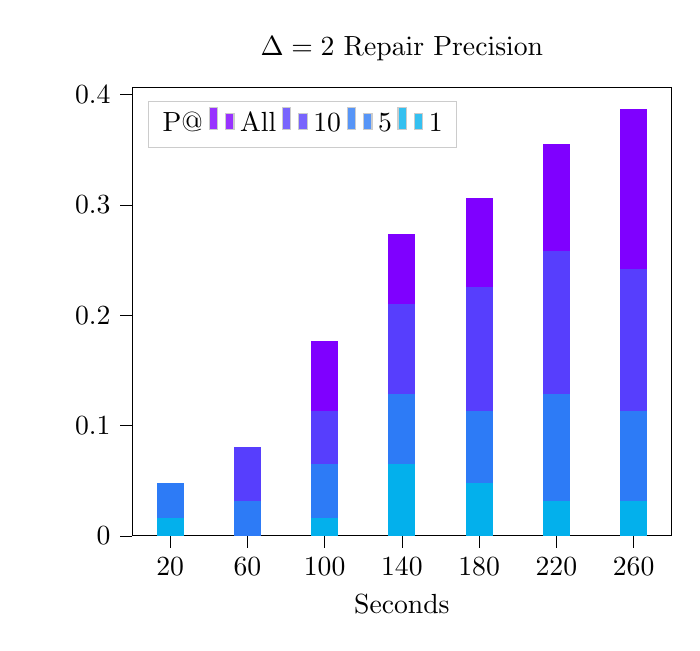
\begin{tikzpicture}

\definecolor{darkgray176}{RGB}{176,176,176}
\definecolor{darkviolet1270255}{RGB}{127,0,255}
\definecolor{deepskyblue3176236}{RGB}{3,176,236}
\definecolor{dodgerblue45123246}{RGB}{45,123,246}
\definecolor{lightgray204}{RGB}{204,204,204}
\definecolor{royalblue8762253}{RGB}{87,62,253}

\begin{axis}[
legend cell align={left},
legend style={fill opacity=0.8, draw opacity=1, text opacity=1, draw=lightgray204, legend columns=-1, legend pos=north west},
tick align=outside,
tick pos=left,
title={$\Delta=2$ Repair Precision},
x grid style={darkgray176},
xlabel={Seconds},
xmin=-0.4925, xmax=6.4925,
xtick style={color=black},
xtick={0,1,2,3,4,5,6},
xticklabels={20,60,100,140,180,220,260},
y grid style={darkgray176},
ylabel={\phantom{Precision@k}},
ymin=0, ymax=0.40635,
ytick style={color=black}
]
\addlegendimage{empty legend}
\addlegendentry{P@}
\draw[draw=none,fill=darkviolet1270255] (axis cs:-0.175,0) rectangle (axis cs:0.175,0.048);
\addlegendimage{ybar,ybar legend,draw=none,fill=darkviolet1270255}
\addlegendentry{All}

\draw[draw=none,fill=darkviolet1270255] (axis cs:0.825,0) rectangle (axis cs:1.175,0.081);
\draw[draw=none,fill=darkviolet1270255] (axis cs:1.825,0) rectangle (axis cs:2.175,0.177);
\draw[draw=none,fill=darkviolet1270255] (axis cs:2.825,0) rectangle (axis cs:3.175,0.274);
\draw[draw=none,fill=darkviolet1270255] (axis cs:3.825,0) rectangle (axis cs:4.175,0.306);
\draw[draw=none,fill=darkviolet1270255] (axis cs:4.825,0) rectangle (axis cs:5.175,0.355);
\draw[draw=none,fill=darkviolet1270255] (axis cs:5.825,0) rectangle (axis cs:6.175,0.387);
\draw[draw=none,fill=royalblue8762253] (axis cs:-0.175,0) rectangle (axis cs:0.175,0.048);
\addlegendimage{ybar,ybar legend,draw=none,fill=royalblue8762253}
\addlegendentry{10}

\draw[draw=none,fill=royalblue8762253] (axis cs:0.825,0) rectangle (axis cs:1.175,0.081);
\draw[draw=none,fill=royalblue8762253] (axis cs:1.825,0) rectangle (axis cs:2.175,0.113);
\draw[draw=none,fill=royalblue8762253] (axis cs:2.825,0) rectangle (axis cs:3.175,0.21);
\draw[draw=none,fill=royalblue8762253] (axis cs:3.825,0) rectangle (axis cs:4.175,0.226);
\draw[draw=none,fill=royalblue8762253] (axis cs:4.825,0) rectangle (axis cs:5.175,0.258);
\draw[draw=none,fill=royalblue8762253] (axis cs:5.825,0) rectangle (axis cs:6.175,0.242);
\draw[draw=none,fill=dodgerblue45123246] (axis cs:-0.175,0) rectangle (axis cs:0.175,0.048);
\addlegendimage{ybar,ybar legend,draw=none,fill=dodgerblue45123246}
\addlegendentry{5}

\draw[draw=none,fill=dodgerblue45123246] (axis cs:0.825,0) rectangle (axis cs:1.175,0.032);
\draw[draw=none,fill=dodgerblue45123246] (axis cs:1.825,0) rectangle (axis cs:2.175,0.065);
\draw[draw=none,fill=dodgerblue45123246] (axis cs:2.825,0) rectangle (axis cs:3.175,0.129);
\draw[draw=none,fill=dodgerblue45123246] (axis cs:3.825,0) rectangle (axis cs:4.175,0.113);
\draw[draw=none,fill=dodgerblue45123246] (axis cs:4.825,0) rectangle (axis cs:5.175,0.129);
\draw[draw=none,fill=dodgerblue45123246] (axis cs:5.825,0) rectangle (axis cs:6.175,0.113);
\draw[draw=none,fill=deepskyblue3176236] (axis cs:-0.175,0) rectangle (axis cs:0.175,0.016);
\addlegendimage{ybar,ybar legend,draw=none,fill=deepskyblue3176236}
\addlegendentry{1}

\draw[draw=none,fill=deepskyblue3176236] (axis cs:0.825,0) rectangle (axis cs:1.175,0);
\draw[draw=none,fill=deepskyblue3176236] (axis cs:1.825,0) rectangle (axis cs:2.175,0.016);
\draw[draw=none,fill=deepskyblue3176236] (axis cs:2.825,0) rectangle (axis cs:3.175,0.065);
\draw[draw=none,fill=deepskyblue3176236] (axis cs:3.825,0) rectangle (axis cs:4.175,0.048);
\draw[draw=none,fill=deepskyblue3176236] (axis cs:4.825,0) rectangle (axis cs:5.175,0.032);
\draw[draw=none,fill=deepskyblue3176236] (axis cs:5.825,0) rectangle (axis cs:6.175,0.032);
\end{axis}

\end{tikzpicture}
}
  \caption{Latency benchmarks. Note the varying axis ranges. The red line marks Seq2Parse and the orange line marks BIFI's Precision@1 on the same repairs.}\label{fig:human}
\end{figure}